\section{VCO: Voltage Controlled Oscillator}
Esta secci\'on se propone el dise\~no de un oscilador de se\~nales senoidales cuya frecuencia pueda ser controlada por una tensi\'on de entrada,
de forma tal que para un dado rango de tensiones, se pueda producir la se\~nal deseada que var\'ie en un rango esperado de frecuencias.
En la Fig. \ref{fig:esquema_general_ejercicio_3} se ilustra un esquema general del sistema deseado.

\begin{figure}[H]
    \centering
    \includegraphics[scale=0.5]{../EJ3/Recursos/system_scheme.png}
    \caption{Esquema general del sistema propuesto}
    \label{fig:esquema_general_ejercicio_3}
\end{figure}


\subsection{Introducci\'on te\'orica}
El objetivo de esta introducci\'on es establecer las bases te\'oricas sobre las cuales se construye
el an\'alisis desarrollado para el dise\~no del sistema propuesto. No obstante, se asume que el lector posee
una base te\'orica sobre algunos conceptos, lo cual se ir\'a indicando a lo largo de tal an\'alisis.

\subsubsection{Distorsi\'on Arm\'onica}
La teor\'ia de series generalizadas de Fourier establece que cualquier se\~nal peri\'odica, es decir una funci\'on dada tal que
$f: I\!R -> I\!R$ que cumple tener un per\'iodo fundamental dado $f(t + T) = f(t)$, con T perteneciente a los reales positivos, puede
ser proyectada sobre un espacio vectorial descripto por su base ortonormal.
En otras palabras, la serie trigonométrica de Fourier como caso particular permite describir un se\~nal peri\'odica como combinaci\'on 
lineal de funciones seno y coseno. Se suele denominar a cada una de estas componentes como arm\'onicos cuyas frecuencias son m\'ultiplos de la 
frecuencia fundamental, y desde un punto de vista espectral se puede observar la distribuci\'on de potencia de la se\~nal para cada frecuencia
arm\'onica.

\begin{figure}[H]
    \centering
    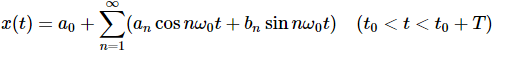
\includegraphics[scale=0.6]{../EJ3/Recursos/fourier_series.PNG}
    \caption{Series de Fourier}
\end{figure}


\begin{figure}[H]
    \centering
    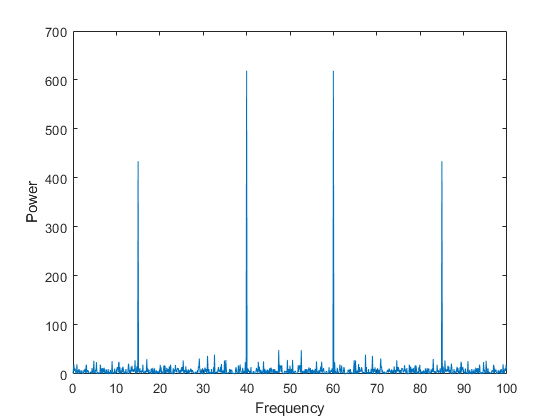
\includegraphics[scale=0.4]{../EJ3/Recursos/BasicSpectralAnalysisExample_01.png} 
    \caption{Espectro en frecuencia}
\end{figure}

La distorsi\'on arm\'onica puede ser entendida como la presencia de arm\'onicos no deseados que en el dominio temporal alteran o distorsionan la forma
de onda esperada, esto puede pasar como consecuencia del uso de sistemas no lineales o por el l\'imite f\'isico de ancho de banda que suelen tener
los circuitos, aunque no siempre se vuelve apreciable su efecto sobre la eliminaci\'on de los arm\'onicos deseados.
As\'i, una se\~nal senoidal pura \'unicamente contiene su arm\'onico fundamental, y en t\'erminos del espectro en frecuencia s\'olo una componente. Esto permite
estudiar la distorsi\'on de tales se\~nales analizando aquellos componentes arm\'onicos no deseados que pueden aparecer, y se utiliza la expresi\'on de la Ec. \ref{eq:distorsion_de_armonico}
para cuantificarla. La distorsi\'on total se define como se observa en la Ec. \ref{eq:total_distorsion}.

\begin{equation}
    HD_n = \frac{RMS_n}{RMS_{fund}}
    \label{eq:distorsion_de_armonico}
\end{equation}

\begin{equation}
    THD = \sqrt{\sum_{n} (HD_n)^{2}}
    \label{eq:total_distorsion}
\end{equation}

\subsubsection{Jitter}
Se define el Jitter como la desviaci\'on pr\'actica del per\'iodo de una se\~nal respecto de su valor te\'orico esperado. Este es un aspecto
a tener en cuenta en el dise\~no y an\'alisis de osciladores, y puede clasificarse generalmente seg\'un si es aleatorio o determin\'istico.

\begin{figure}[H]
    \centering
    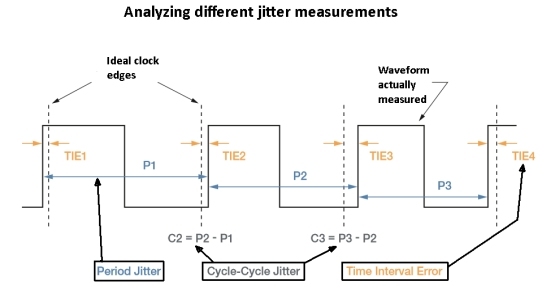
\includegraphics[scale=0.5]{../EJ3/Recursos/different-jitter-measurements.jpg}
    \caption{Diagrama del Jitter medido en un per\'iodo o entre ciclos}
    \label{fig:jitter_diagram}
\end{figure}

El jitter aleatorio corresponde a la desviaci\'on del per\'iodo provocada por el ruido t\'ermico que generan los componentes resistivos en la pr\'actica.
Por otro lado, el jitter determin\'istico consiste en analizar las posibles desviaciones temporales, ya sea de un per\'iodo respecto del valor real, as\'i
como entre per\'iodos de ciclos consecutivos. Esto puede observarse en la Fig. \ref{fig:jitter_diagram}.

\subsection{An\'alisis de circuitos}
Se busca realizar un an\'alisis de los circuitos empleados posteriormente en el dise\~no para facilitar, no s\'olo este proceso,
sino la divisi\'on en etapas seg\'un lo requiera el sistema, teniendo en cuenta las fortalezas y debilidades de cada una de ellas.

\subsubsection{Acondicionamiento lineal de se\~nal}
En la pr\'actica suele ser necesario realizar un acondicionamiento lineal de una se\~nal de entrada, esto implica matem\'aticamente aplicar un desplazamiento
y un escalaje sobre la magnitud de entrada, adaptando el rango de valores de entrada a un rango aceptable de salida. Se propone como circuito para realizar esta transformaci\'on
de las magnitudes, el ilustrado en la Fig. \ref{fig:circuito_acondicionamiento_lineal}.

\begin{figure}[H]
    \centering
    \includegraphics[scale=0.55]{../EJ3/Recursos/circuito_acondicionamiento_lineal.png}
    \caption{Acondicionamiento lineal de se\~nales}
    \label{fig:circuito_acondicionamiento_lineal}
\end{figure}

Se plantean las siguientes ecuaciones, donde se define la salida del amplificador operacional configurado como buffer o seguidor de tensi\'on $V_{OFF}$.

\begin{align*}
    & V_{OFF} = \frac{V_{CC} \cdot R_2}{R_1 + R_2} \\
    & V_o = V_i \cdot \frac{R_4}{R_3 + R_4} \cdot \frac{R_5 + R_6}{R_5}
    + V_{OFF} \cdot \frac{R_3}{R_3 + R_4} \cdot \frac{R_5 + R_6}{R_5}
\end{align*}

Aplicando como criterio para simplificar el manejo algebraico, resulta pr\'actico establecer que se cumpla la condici\'on
$R_3 = R_5$ y $R_4 = R_6$.

\begin{equation}
    V_o = V_i \cdot \frac{R_4}{R_5} + V_{OFF}
\end{equation}

En conclusi\'on, este circuito con esta \'ultima expresi\'on permite de manera sencilla realizar una transformaci\'on que permita adaptar o acondicionar
la se\~nal entrante, conociendo la pendiente y ordenada al origen que se desean como salida. Es importante mencionar que el circuito no garantiza un l\'imite de tensi\'on 
que no sea el de saturaci\'on de los amplificadores, con lo cual a menos que se haga uso de este, ser\'a necesario un circuito limitador de tensi\'on en la salida seg\'un el caso.

\subsubsection{Comparador Schmitt Trigger inversor}
El comparador Schmitt Trigger es una configuraci\'on del amplificador operacional utilizando una realimentaci\'on regenerativa o positiva,
que lo que busca es crear un comparador con hist\'eresis para prevenir fluctuaciones u oscilaciones en la salida del mismo por el efecto de se\~nales
con contenido no deseado de ruido. Estas configuraciones vienen en la forma de inversoras o no inversoras, y establecen dos l\'imites de comparaci\'on
para determinar estado alto o estado bajo, y cuando no se emplea un corrimiento por offset, se encuentran sim\'etricos al cero.

\begin{figure}[H]
    \centering
    \includegraphics[scale=0.7]{../EJ3/Recursos/diagrama_schmitt_trigger.png}
    \caption{Diagrama del comparador con hist\'eresis}
    \label{fig:diagrama_schmitt_trigger}
\end{figure}

En la Fig. \ref{fig:diagrama_schmitt_trigger} se puede observar la funci\'on de $V_o = f(V_i)$ del comparador Schmitt Trigger inversor,
para el cual se propone el circuito de la Fig. \ref{fig:circuito_schmitt_trigger}.

\begin{figure}[H]
    \centering
    \includegraphics[scale=0.6]{../EJ3/Recursos/schmitt_trigger.png}
    \caption{Circuito Schmitt Trigger inversor}
    \label{fig:circuito_schmitt_trigger}
\end{figure}

Se plantea el potencial en las dos entradas del amplificador operacional, y dado que la transici\'on se da en torno al encuentro
de ambos valores de tensi\'on, se igualan las expresiones y asumiendo estados alto y bajo de salida, se encuentra la expresi\'on
de los valores de comparaci\'on.

\begin{align*}
    & V^{+} = V_o \cdot \frac{R_1}{R_1 + R_2} \\
    & V^{-} = V_i \\
    & \Rightarrow V_T = V_{CC_{SAT}} \cdot \frac{R_1}{R_1 + R_2}
\end{align*}

Es importante observar que se considera que el amplificador operacional no es Rail-To-Rail, dado que se usa que la salida de estado alto o bajo
est\'a dada por la saturaci\'on de la salida, con lo cual es necesario tener en cuenta este aspecto en el momento del dise\~no para evitar desviaciones pr\'acticas
por tener en cuenta de forma incorrecta un valor alto o bajo de tensi\'on de salida.

\subsubsection{Voltage Controlled Oscillator}
En la Fig. \ref{fig:circuito_vco} se puede observar el circuito propuesto para realizar el armado de un VCO utilizando dos amplificadores operacionales
y un MOSFET. Se realiza un an\'alisis considerando un comportamiento ideal de los amplificadores, y asumiendo que el lector tiene un conocimiento del 
funcionamiento del transistor.

\begin{figure}[H]
    \centering
        \includegraphics[scale=0.5]{../EJ3/Recursos/circuit_vco.png}
    \caption{Circuito de un Voltage Controlled Oscillator}
    \label{fig:circuito_vco}
\end{figure}

\paragraph{Operaci\'on del circuito:} Se utiliza una configuraci\'on de amplificador operacional para poder integrar una se\~nal cuadrada,
de esta forma se produce una se\~nal triangular, no obstante, para poder garantizar que la frecuencia sea controlada por la tensi\'on de entrada,
el valor de corriente que determina los tiempos de carga y descarga depende de la tensi\'on de entrada. De esta forma, a corriente constante la carga del capacitor
se da linealmente hasta encontrarse con los extremos de comparaci\'on de la configuraci\'on schmitt trigger inversora, que produce en funci\'on de ello una onda
cuadrada sincronizada que conmuta un transistor para lograr cambiar el sentido de corriente, y por ende, de carga del capacitor.

\paragraph{Comparador Schmitt Trigger inversor:} De la comprensi\'on cualitativa del funcionamiento del VCO, se puede ver que el comparador
produce una onda cuadrada a partir de la triangular, pero adem\'as su funcionalidad principal est\'a en determinar el valor pico de tensi\'on de la onda triangular.
Sea $V_x$ la tensi\'on pico de la triangular, luego se puede determinar este valor utilizando el an\'alisis ya hecho del schmitt trigger, entonces:

\begin{equation}
    V_x = V_{CC_{SAT}} \cdot \frac{R_6}{R_6 + R_7}
    \label{eq:ecuacion_tensiones_vco}
\end{equation}

Es importante notar que las desviaciones pr\'acticas estar\'an dadas por el valor de saturaci\'on que se vea en la salida del amplificador.

\paragraph{Integrador controlado por tensi\'on:} Si inicialmente se ignora la presencia del MOSFET y se lo considera una llave ideal, asumiendo que $R_2 = R_3$,
luego se puede determinar que la corriente $I_{R_1} = \frac{V_i}{2 \cdot R_1}$ se mantiene siempre constante, y cuando la llave est\'e conectada circular\'a por $R_4$ una corriente $I_{R_4} = \frac{V_i}{2 \cdot R_4}$. Dado que el capacitor se carga con una corriente $I_C = I_{R_1} - I_{R_4}$, luego
se deduce que $R_4 = \frac{R_1}{2}$, dado que de esta forma se cumplir\'a que la llave al estar conectada o no, s\'olo cambia el sentido de la corriente del capacitor,
pero su magnitud se mantiene constante. De esta forma se integra y calcula la tensi\'on de salida como:

\begin{equation*}
    i_c(t) = C \cdot \frac{\delta V_c(t)}{\delta t} \Rightarrow \int_0^{t} \delta V_c(t) = \int_0^{t} \frac{i_C(t) \cdot \delta_t}{C}
\end{equation*}

\begin{equation}
    V_c(t) = V_c(0) + \frac{i_C}{C} \cdot t \Rightarrow V_c(t) = V_c(0) + \frac{V_i}{2 \cdot R_1 \cdot C} \cdot t
\end{equation}

\paragraph{Expresi\'on del VCO:} Finalmente, considerando que tal pendiente est\'a dada por el cociente entre la tensi\'on pico a pico
de la triangular y la mitad de su per\'iodo, se puede despejar una expresi\'on que vincula linealmente la tensi\'on de entrada con la frecuencia de la se\~nal de salida. Esto es, la ecuaci\'on que caracterizar\'a el funcionamiento
del VCO.

\begin{equation*}
    \frac{V_{PP} \cdot 2}{T} = \frac{V_i}{2 \cdot C \cdot R_1}
\end{equation*}

\begin{equation}
    f = V_i \cdot \frac{1}{8 \cdot V_x \cdot R_1 \cdot C}
    \label{eq:ecuacion_caracteristica_vco}
\end{equation}

\paragraph{Comentarios pr\'acticos:} Para el circuito propuesto se desea utilizar un transistor de tecnolog\'ia MOSFET dado que de esta forma se garantiza que operando en regi\'on lineal,
la resistencia del canal formado ser\'a peque\~na en comparaci\'on con $R_4$, logrando as\'i que el error por asimetr\'ia de la onda introducido como consecuencia de una asimetr\'ia entre las corrientes
de carga y descarga, sea peque\~no. Por otro lado, no se utiliza un transistor bipolar de juntura o BJT, porque en su modo de conmutaci\'on introducir\'ia un error por la p\'erdida de tensi\'on de la $VCE_{SAT}$, adem\'as
de que al emplear fuente de alimentaci\'on partida, la cuadrada tiene su estado bajo con tensi\'on negativa y podr\'ia superar la tensi\'on de ruptura de la juntura base-emisor, quemando el transistor.

\paragraph{Observaciones:} Durante el an\'alisis te\'orico del circuito, se observ\'o que las limitadas funcionalidades que se le dan al generador a dise\~nar podr\'ian se expandidas. En otras palabras,
podr\'ia emplearse una llave selectora de capacitores m\'ultiplos por 10 entre s\'i, logrando as\'i cambiar el rango de frecuencias a generar. Por otro lado, se podr\'ian colocar etapas de salida de las ondas
generadas para poder modificar la amplitud y el nivel de continua u offset. Finalmente, para modificar el duty de la onda cuadrada o la simetr\'ia de la onda triangular bastar\'ia
con utilizar un preset o potenciometro para modificar las corrientes en las mallas de entrada.

\subsubsection{Conversor triangular a senoidal}

\paragraph{Concepto general:} En t\'erminos te\'oricos, el proceso de conversi\'on de una se\~nal triangular a senoidal es una transformaci\'on que puede ser procesada por un sistema
cuya funci\'on transferencia no lineal debe ser como se describe en la Ec. \ref{eq:modelo_matematico_conversor}. En otras palabras, se debe modelizar esta funci\'on la cual realiza
un mapeo de la se\~nal lineal de entrada sobre el senoide de salida. Es importante destacar, que la frecuencia siempre estar\'a dada por la se\~nal de entrada y la amplitud por el sistema.

\begin{equation}
    X_o = K_1 \cdot \sin{(K_2 \cdot X_i)}
    \label{eq:modelo_matematico_conversor}
\end{equation}

\paragraph{Modelo circuital te\'orico:} En Junio de 1976, Robert G. Meyer, Willy Sanken, y otros colaboradores publicaron un paper en IEEE sobre una investigaci\'on que llevaron a cabo por sugerencia de un colega, sobre la posibilidad de implementar esta funci\'on
descripta anteriormente, empleando un amplificador diferencial con transistores bipolares de juntura. En la Fig. \ref{fig:conversor_teorico_meyer} se puede observar el esquema te\'orico propuesto.

\begin{figure}[H]
    \centering
    \includegraphics[scale=0.5]{../EJ3/Recursos/conversor_teorico_meyer.png}
    \caption{Circuito te\'orico del conversor de Meyer}
    \label{fig:conversor_teorico_meyer}
\end{figure}

En forma sintetizada, se puede demostrar que la corriente que circula por la resistencia $R$ sigue un comportamiento en funci\'on de la tensi\'on de entrada que se ve descripto
por una ecuaci\'on con una funci\'on logar\'itmica. Si se calculan las series de Taylor de dicha funci\'on logar\'itmica y de la funci\'on inversa del seno,
luego se puede encontrar que ambas funciones pueden, bajo ciertas condiciones, compartir los primeros cinco t\'erminos de tales series, con lo cual se obtendr\'ia una aproximaci\'on senoidal. 
Para lograr esto \'ultimo, Meyer dedujo que era necesario que se cumpliera:

\begin{align}
    & I \cdot R \approx 2.5 \cdot V_T \\
    & V_{i_{P}} = V_T \cdot 6.6 \\
    & V_T = \frac{k_B \cdot T}{q}
\end{align}


En conclusi\'on, si se logra que la entrada del circuito sea una se\~nal triangular de simetr\'ia $50\%$ con una tensi\'on pico de $172mV$, donde $I \cdot R \approx 62.5mV$. Entonces,
siguiendo estrictamente esas condiciones en los t\'erminos ideales del modelo circuital propuesto, se puede conseguir una salida senoidal con una distorsi\'on arm\'onica por debajo de $1\%$.

\paragraph{Modelo circuital pr\'actico:} Para que el circuito y las conclusiones anteriores sean aplicables en la realidad, es necesario realizar algunas modificaciones. Estas modificaciones
fueron realizadas bajo ciertos criterios, seg\'un se enumeran a continuaci\'on:

\begin{itemize}
    \item \textbf{Atenuador:} Las se\~nales triangulares conectadas, si bien deben ser de simetr\'ia $50\%$, su amplitud podr\'a variar con lo cual es necesario una etapa de ajuste para 
    llevar el valor de entrada a los $172mV$ necesario para minimizar la distorsi\'on.
    \item \textbf{Par diferencial:} Como se describi\'o anteriormente, es necesario un par diferencial con el cual, bajo ciertas condiciones, aproximar la respuesta de una se\~nal senoidal utilizando como resistencia $R$
    del modelo te\'orico de Meyer. El modelo te\'orico de Meyer emplea una resistencia entre emisores de una etapa diferencial con dos fuentes de corrientes que idealmente son iguales, esto implica en la pr\'actica una complejidad y un costo
    que deben evitarse, con lo cual para ello se utiliza a modo de polarizaci\'on una resistencia $R_8$, que si bien podr\'ia ser una fuente de corriente esto implicar\'ia introducir singularidades en la respuesta en frecuencia que agregar\'ian
    distorsi\'on no buscada. Las resistencias $R_6$ y $R_7$ son utilizadas para generar el mismo efecto que la $R$ entre emisores del modelo te\'orico de Meyer, no obstante se conectan de esta forma porque es necesario que lo que antes eran dos fuentes de corriente,
    ahora sea una s\'ola resistencia que provee $2 \cdot I$.
    \item \textbf{Fuente de corriente espejo proporcional:} Se la emplea como carga activa porque as\'i se logra mejorar la relaci\'on sim\'etrica entre corrientes de $Q_1$ y $Q_2$ y crear idealmente un punto de tierra virtual en el colector de $Q_2$,
    lo que permite tener una salida en modo com\'un. Y dado que en el modelo incremental la resistencia de tal fuente es muy grande, las corrientes incrementales se van mayoritariamente por la salida, caracterizando al amplificador
    por tener una salida de corriente. Se busca que $R_4 = R_5$, emulando una fuente espejo simple, no obstante la desviaci\'on por diferencia en curvas caracter\'isticas de las junturas
    es menor con respecto al par espejo simple.
    \item \textbf{Etapa amplificador de transimpedancia:} Se utiliza un amplificador de transimpedancia aprovechando que la salida del diferencial con carga activa es de corriente, y dado que la salida est\'a montada sobre una tierra virtual,
    luego no es necesario realizar ning\'un ajuste sobre el nivel de continua u offset. La ganancia del amplificador estar\'a dada por $-R_{10}$.
\end{itemize}

\begin{figure}[H]
    \centering
    \includegraphics[scale=0.4]{../EJ3/Recursos/conversor_propuesto.png}
    \caption{Conversor triangular a senoidal propuesto}
    \label{fig:circuito_conversor_propuesto}
\end{figure}

\paragraph{Comentarios pr\'acticos:} El an\'alisis del funcionamiento del par diferencial asume condiciones ideales y que los $Q_1$ y $Q_2$ son transistores iguales. No obstante,
en la realidad podr\'ia suceder que no lo sean, y a pesar de que ambos transistores tienen mismas mallas de entrada, puede suceder que dado las diferencias entre sus curvas de polarizaci\'on,
luego sus corrientes no sean iguales. Esto producir\'ia una asimetr\'ia en el par diferencia que provocar\'ia un corrimiento en la salida. Para solucionar esto en caso de que en la pr\'actica se presenten
dispersiones grandes, se suele utilizar un preset para compensar esa desigualdad. No obstante, con el objetivo de minimizar la cantidad de presets para calibraci\'on usados, se propone el siguiente circuito
como alternativa.

\begin{figure}[H]
    \centering
    \includegraphics[scale=0.6]{../EJ3/Recursos/compensacion_activa.png}
    \caption{Compensaci\'on activa de diferencias entre $Q_1$ y $Q_2$}
    \label{fig:compensacion_activa}
\end{figure}

El circuito de la Fig. \ref{fig:compensacion_activa} es una propuesta para compensar de forma activa las diferencias producidas por las diferencias
entre las junturas de ambos transistores $Q_1$ y $Q_2$. El objetivo es, asumiendo que $R_6 = R_7$, luego idealmente el amplificador operacional mantiene la diferencia
de tensi\'on entre las ca\'idas en las resistencias nulo, para lo cual realimenta una tensi\'on de base en el $Q_2$ desplazando su curva caracter\'istica hasta que se encuentre
coincidente con la de $Q_1$. Dado que esta compensaci\'on activa no debe interferir en el circuito incremental, se utiliza un capacitor de gran valor de capacidad para que s\'olo
opere en frecuencias muy bajas o continua.

\subsection{Dise\~no de VCO}

\subsubsection{Especificaciones y etapas}
Se desea dise\~nar un oscilador controlado por tensi\'on cuya salida sea senoidal, y que para el rango de tensiones de 0V a 5V, la salida
var\'ie de 1kHz a 10kHz. A partir de esto, se deduce que es necesario diagramar un sistema como se ilustra en la Fig. \ref{fig:diagrama_en_bloques}.

\begin{figure}[H]
    \centering
    \includegraphics[scale=0.45]{../EJ3/Recursos/diagrama_en_bloques.png}
    \caption{Diagrama en bloques del sistema a dise\~nar}
    \label{fig:diagrama_en_bloques}
\end{figure}

\begin{itemize}
    \item \textbf{Acondicionamiento lineal:} En principio es necesario una etapa para adaptar el rango lineal de tensiones de entrada comprendidas entre
    0 - 5V, a un rango que sea adecuado seg\'un lo necesite el oscilador controlado por tensi\'on, ya que el esquema a utilizar no oscila para 0V de entrada.
    \item \textbf{Oscilador Controlado por Tensi\'on:} Utilizando esta etapa, para un rango deseado de tensiones, se generar\'an ondas cuadradas y triangulares
    que cumplan con la frecuencias deseadas, y en principio no existe limitante alguna sobre las tensiones de las se\~nales a utilizar.
    \item \textbf{Conversor Triangular a Senoidal:} Se utiliza esta etapa para convertir la onda triangular del oscilador en una se\~nal senoidal.
\end{itemize}

\subsubsection{C\'alculo de componentes}
En una primera aproximaci\'on del dise\~no, se busca que el oscilador controlado por tensi\'on genere una frecuencia $f = 1kHz$ para una tensi\'on de entrada
arbitraria que sea mucho mayor que el piso de ruido, y no demasiado grande para garantizar que al multiplicar por 10 esa tensi\'on, la frecuencia luego sea $f = 10kHz$.
Luego, la etapa de acondicionamiento lineal debe ajustar el rango de entrada al rango esperado por el VCO, y finalmente si la salida del oscilador tiene una amplitud mucho mayor
que el piso de ruido, en el conversor triangular a senoidal se aten\'ua y produce una senoidal de tensi\'on pico ajustable.

El problema de esta primera aproximaci\'on es que, 
puede suceder que para distintas frecuencias por los consumos de corriente y el Slew Rate, la tensi\'on de saturaci\'on no se mantenga invariante, produciendo un error 
que puede ser proporcional con la frecuencia de operaci\'on de alguna forma. Entonces, si se dise\~na primero siguiendo la aproximaci\'on antes explicada, se puede encontrar que en la pr\'actica
las desviaciones para la m\'inima frecuencia son menores, pero para la m\'axima frecuencia llegan a ser del $15 \%$, con lo cual tomando dimensi\'on de este error por las limitaciones din\'amicas del amplificador 
operacional, se utiliza una relaci\'on de acondicionamiento de la se\~nal que compense el error por frecuencias.


Es importanta aclarar, que se utilizar\'a como amplificador operacional el TL082, dado que tiene un buen ancho de banda y slew rate, pero adem\'as se lo puede encontrar disponible en tecnlogo\'ia de montaje superficial.

\paragraph{Acondicionamiento Lineal:} Se dise\~na el circuito de la Fig. \ref{fig:circuito_acondicionamiento_lineal}, que en principio deber\'ia estar fijado para conseguir adaptar el rango 0 - 5V a
un rango de 1 - 10V, pero que para compensar el error real por las limitaciones ya mencionadas debe adaptar al rango 1.05 - 11.80V. Si $V_i = 0V \Rightarrow V_o = V_{OFF} = 1.05V$, entonces utilizando resistencias $R_1 = 120k \Omega$ y $R_2 = 9.1k \Omega$ se 
obtiene la tensi\'on de offset. Por otro lado, cuando $m = \frac{11.8V - 1.05V}{5V - 0V} = \frac{R_4}{R_5}$, entonces utilizando resistencias $R_4 = 100k \Omega$ y $R_5 = 47k \Omega$ se satisface la pendiente de tal adaptaci\'on.

\paragraph{Oscilador Controlador por Tensi\'on:} Se dise\~na el circuito de la Fig. \ref{fig:circuito_vco} para cumplir con el criterio de que dada una $V_i = 1V \Rightarrow f = 1kHz$. En primer lugar, por tomar un valor arbitrario,
se decide utilizar una triangular de valor pico $V_x = 5V$, con lo cual asumiendo que $V_{CC_{SAT}} = 12.5V$ siempre que la alimentaci\'on sea $V_{CC} = -V_{EE} = 15V$, se utilizan $R_6 = 1k \Omega $ y $R_7 = 1.5k \Omega $. Luego de forma arbitraria, $R_2 = R_3 = 1k \Omega$, dado que lo importante
es que cumplan la relaci\'on de igualdad. Finalmente, empleando la Ec. \ref{eq:ecuacion_caracteristica_vco}, para conseguir tal frecuencia se propone $C = 8.2 nF$ y $R_1 = 3k \Omega \Rightarrow R_4 = 1.5k \Omega$.

\paragraph{Conversor triangular a senoidal:} Se dise\~na el circuito de la Fig. \ref{fig:circuito_conversor_propuesto}. Utilizando $R_1 = 2.4k \Omega$, $R_2 = 50k \Omega$ y $R_3 = 1k \Omega$, que provienen de plantear un rango de atenuaci\'on
de la se\~nal de entrada que se encuentra entre el $1\%$ y el $30\%$. Luego, para los pares NPN se usa el BC547 y para los pares PNP se usa el BC557, y $R_9 = 1k \Omega$ para cumplir con las condiciones de simetr\'ia del par diferencial.
El circuito se arm\'o de esta manera en la pr\'actica para determinar si hab\'ia alguna disparidad entre las corrientes de ambos transistores y si, en ese caso, era necesaria la compensaci\'on activa propuesto. Finalmente,
se encontr\'o que tal compensaci\'on no era necesaria porque el par empleado coincid\'ia lo suficiente.

Para el dise\~no del par diferencial se inicia planteando que $R_6 = R_7 = 47 \Omega$, luego como son transistores con un $hFE >> 1$ entonces se puede despreciar las corrientes de base,
asumiendo as\'i en la malla de polarizaci\'on que:

\begin{align*}
    & V_{EE} + R_8 \cdot 2 \cdot I + I \cdot R_7 + V_{BE} = 0 \\
    & \Rightarrow R_8 = \frac{-V_{EE} - V_{BE} - R_7 \cdot I}{2 \cdot I}
\end{align*}

Luego, con una resistencia de $47 \Omega$, para cumplir la relaci\'on deducida por Meyer, es necesario una corriente de $I = 664.89 \mu A$, con lo cual
de la ecuaci\'on anterior se deduce que $R_8 = 11k \Omega$. Finalmente, en el par espejo se utilizan $R_4 = R_5 = 3.3 k \Omega$ para tener una corriente igual en cada rama,
y no tener mucha ca\'ida de tensi\'on que produzca la saturaci\'on de alg\'un transistor. La $R_{10}$ es un preset variable de $50 k \Omega$ para ajustar la tensi\'on pico de la senoidal
de salida.

\subsubsection{Simulaci\'on y verificaci\'on}
Realizando la simulaci\'on del circuito en LTSpice, se pudo verificar el correcto funcionamiento del circuito total tal como es esperado,
en las Figs. \ref{fig:verificacion} se ilustran el acondicionamiento del rango de tensiones de entrada y una oscilaci\'on del oscilador y el conversor.

\begin{figure}[H]
    \centering
    \begin{tabular}{c c}
        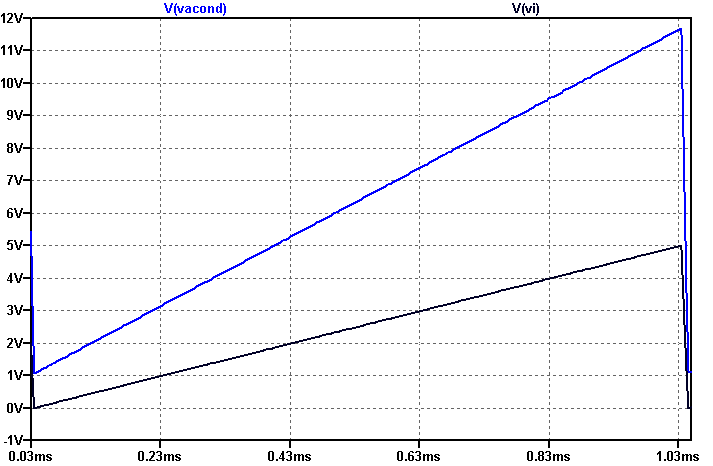
\includegraphics[scale=0.35]{../EJ3/Recursos/verificacion_acondicionamiento.png} &
        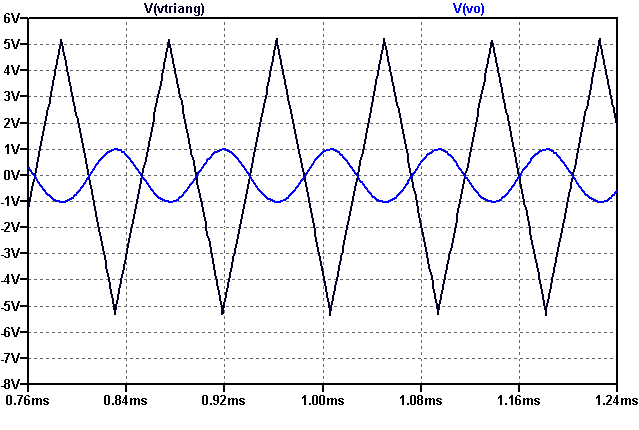
\includegraphics[scale=0.4]{../EJ3/Recursos/verificacion_vco.png}
    \end{tabular}
    \caption{Verificaci\'on del acondicionamiento y oscilaci\'on}
    \label{fig:verificacion}
\end{figure}

\subsection{Resultados}

\subsubsection{Funcionamiento}
Se miden las diferentes se\~nales generadas por el oscilador controlado por tensi\'on, en los casos l\'imite de la entrada de tensi\'on, as\'i
verificando el funcionamiento con las frecuencias y amplitud deseada.

\begin{figure}[H]
    \centering
    \begin{tabular}{c c}
        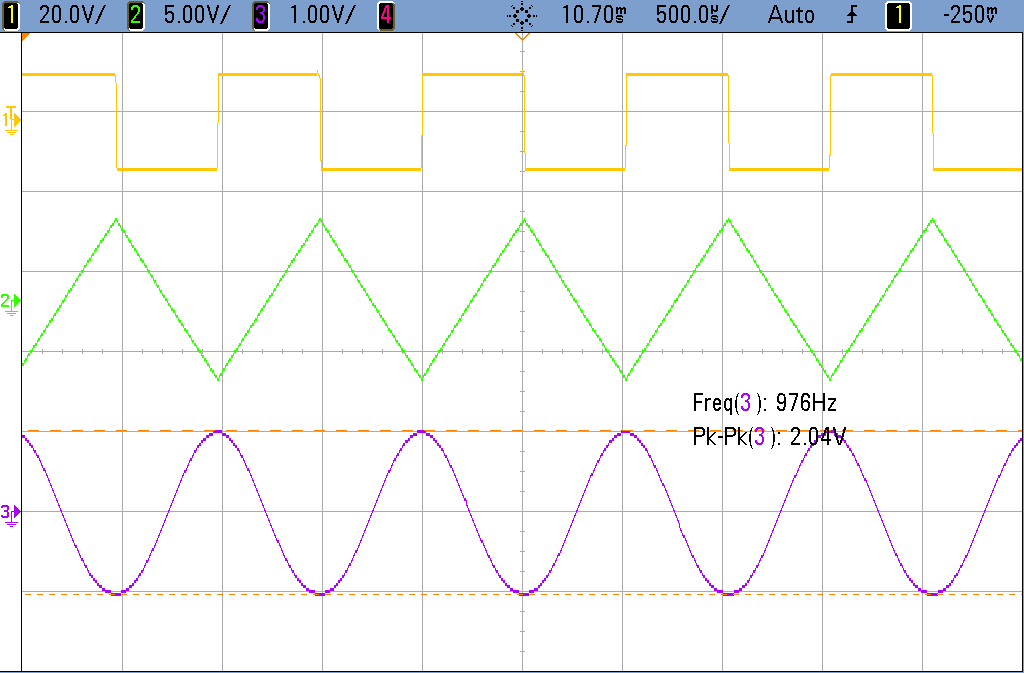
\includegraphics[scale=0.2]{../EJ3/Mediciones/Actuales/Osciloscopio/Distorsion_1k/cropped_scope_0.png} & 
        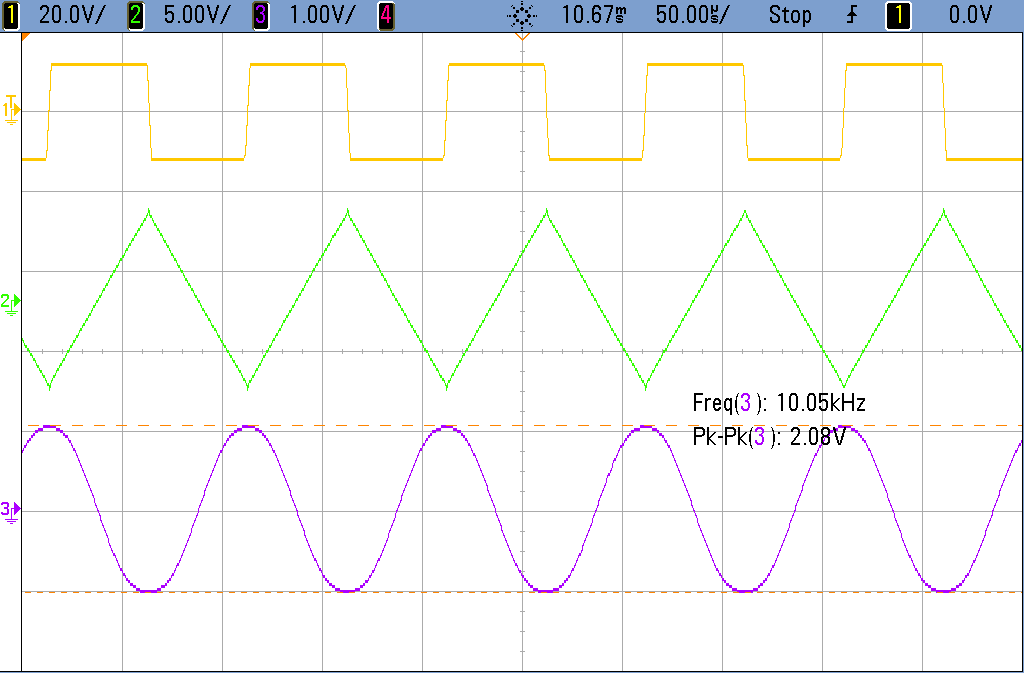
\includegraphics[scale=0.2]{../EJ3/Mediciones/Actuales/Osciloscopio/Distorsion_10k/cropped_scope_13.png} 
    \end{tabular}
    \caption{Medici\'on de se\~nal cuadrada, triangular, senoidal del VCO con casos $V_i = 0V$ y $V_i = 5V$}
    \label{fig:mediciones_funcionamiento}
\end{figure}

\subsubsection{Distorsi\'on Arm\'onica}
Para la determinaci\'on de la distorsi\'on arm\'onica total de la senoidal generada por el oscilador, es necesario medir la transformada Fourier
para analizar la composici\'on espectral de la se\~nal y analizar la magnitud de los arm\'onicos no deseados que componen a la distorsi\'on mencionada.
Para ello se utiliza la transformada r\'apida de Fourier con el osciloscopio y se obtiene:

\begin{figure}[H]
    \centering
    \begin{tabular}{c c}
        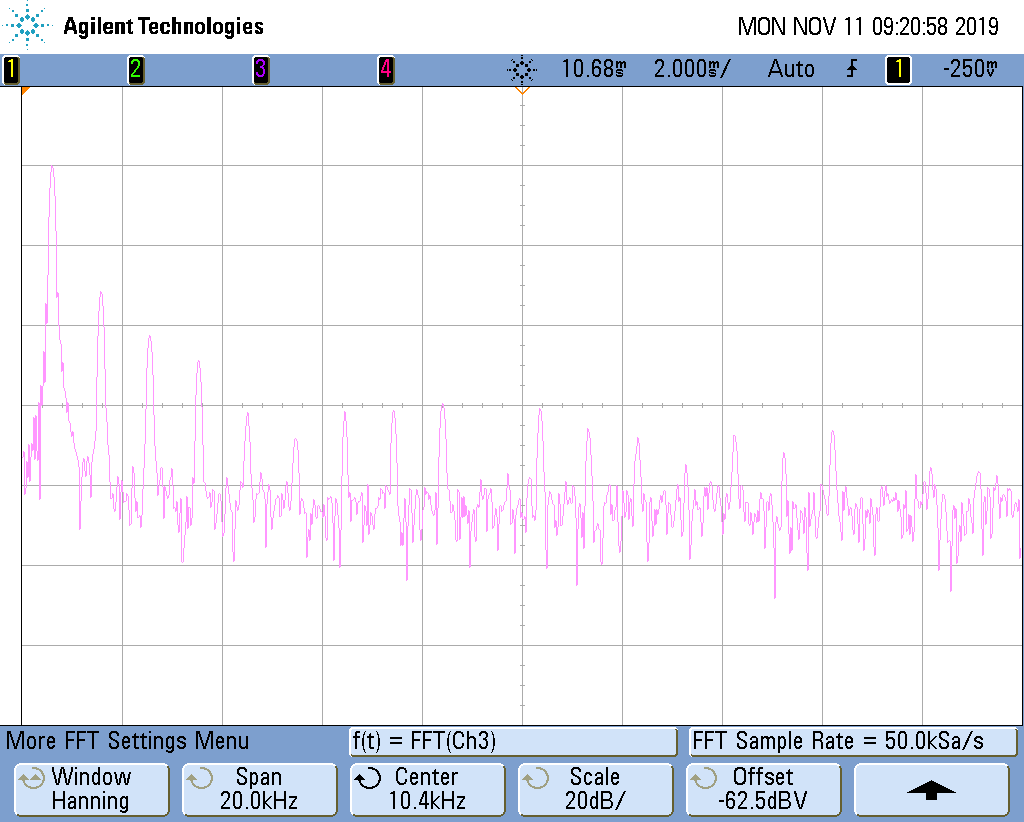
\includegraphics[scale=0.2]{../EJ3/Mediciones/Actuales/Osciloscopio/Distorsion_1k/scope_2.png} &
        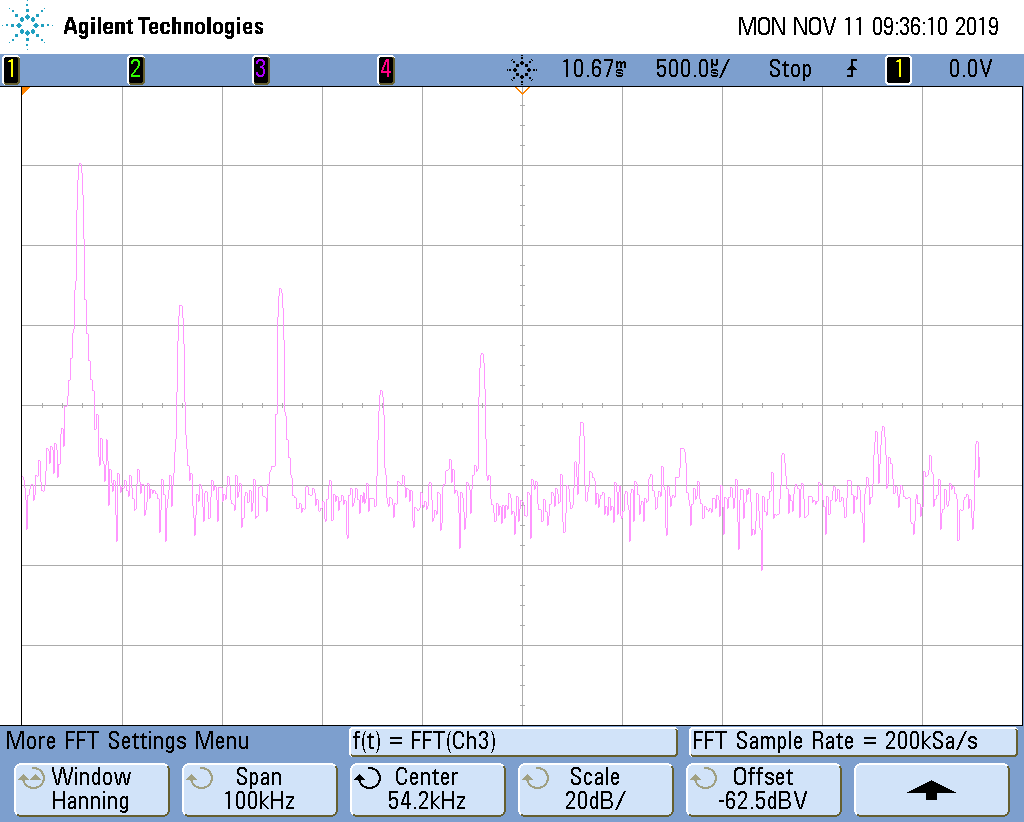
\includegraphics[scale=0.2]{../EJ3/Mediciones/Actuales/Osciloscopio/Distorsion_10k/scope_11.png}
    \end{tabular}
    \caption{Medici\'on de la FFT de la se\~nal senoidal. En la izquierda para $f = 1kHz$ y en la derecha $f = 10kHz$}
\end{figure}

\begin{table}[H]
    \centering
    \begin{tabular}{c c c}
        $f [Hz]$ & $A [dBV]$ & $A [V^{2}]$ \\
        \hline \\
        $1k$ & $-4.58$ & $0.348$ \\
        $2k$ & $-40.5$ & $8.95 \cdot 10^{-5}$ \\
        $3k$ & $-59.8$ & $1.05 \cdot 10^{-6}$ \\
        $4k$ & $-75.1$ & $3.08 \cdot 10^{-8}$ \\
        $5k$ & $-85.3$ & $2.94 \cdot 10^{-9}$ \\
        $6k$ & $-86.7$ & $2.14 \cdot 10^{-9}$ \\
        $7k$ & $-85$ & $3.16 \cdot 10^{-9}$ \\
        $8k$ & $-93.1$ & $4.89 \cdot 10^{-10}$ \\
        $9k$ & $-92.1$ & $6.17 \cdot 10^{-10}$ \\
        \hline \\
    \end{tabular}
    \caption{Medici\'on con $f = 1kHz$}
\end{table}

\begin{equation}
    THD_{f = 1kHz} = 1.61 \%
\end{equation}

\begin{table}[H]
    \centering
    \begin{tabular}{c c c}
        $f [Hz]$ & $A [dBV]$ & $A [V^{2}]$ \\
        \hline \\
        $10k$ & $-2.51$ & $0.56$ \\
        $20k$ & $-36.9$ & $0.000205$ \\
        $30k$ & $-33.7$ & $0.0004$ \\
        $40k$ & $-58.6$ & $1.38 \cdot 10^{-6}$ \\
        $50k$ & $-53.7$ & $4.24 \cdot 10^{-6}$ \\
        $60k$ & $-72.4$ & $5.72 \cdot 10^{-8}$ \\
        $70k$ & $-74.6$ & $3.46 \cdot 10^{-8}$ \\
        $80k$ & $-80.3$ & $9.23 \cdot 10^{-9}$ \\
        $90k$ & $-82.2$ & $6.02 \cdot 10^{-9}$ \\
        \hline \\
    \end{tabular}
    \caption{Medici\'on con $f = 1kHz$}
\end{table}

\begin{equation}
    THD_{f = 10kHz} = 3.36 \%
\end{equation}

\subsubsection{Medida de Jitter}
Para determinar la medida de Jitter, se tomaron mediciones del per\'iodo de la se\~nal en cada caso a lo largo de un determinado
tiempo y luego, utilizando las herramientas del osciloscopio de Quick Measure, se determinaron los valores medios, m\'inimo, m\'aximo y
la desviaci\'on est\'andar. En conclusi\'on, se puede observar la medida del Jitter en la desviaci\'on est\'andar de la medici\'on en la Fig. \ref{fig:medida_jitter}.

\begin{figure}[H]
    \centering
    \begin{tabular}{c c}
        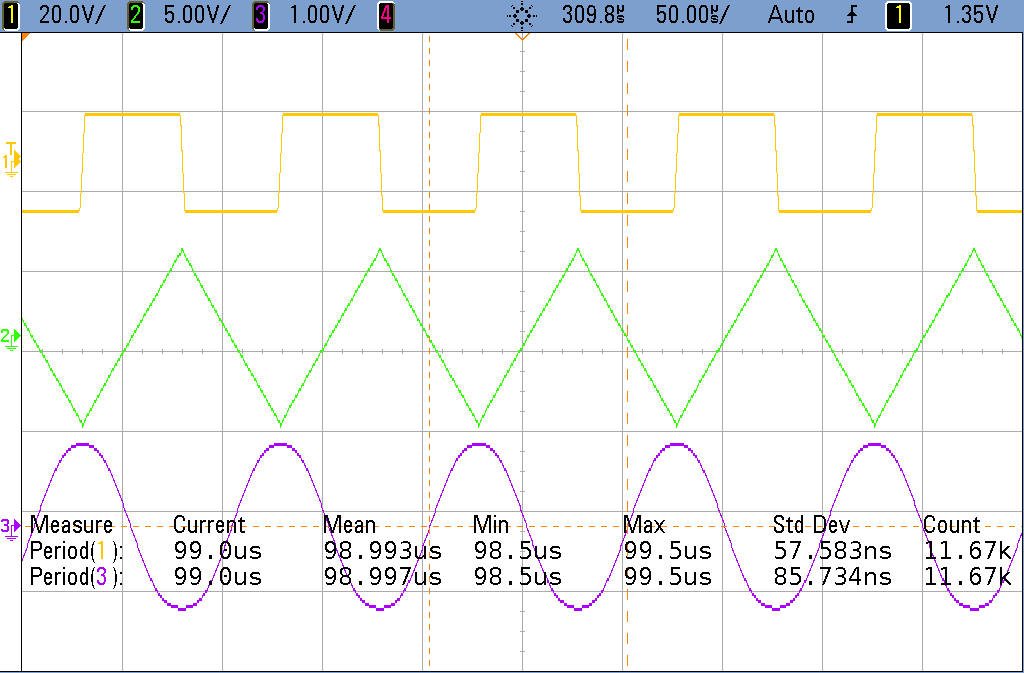
\includegraphics[scale=0.2]{../EJ3/Mediciones/Actuales/Osciloscopio/Jitter/cropped_scope_19.png} &
        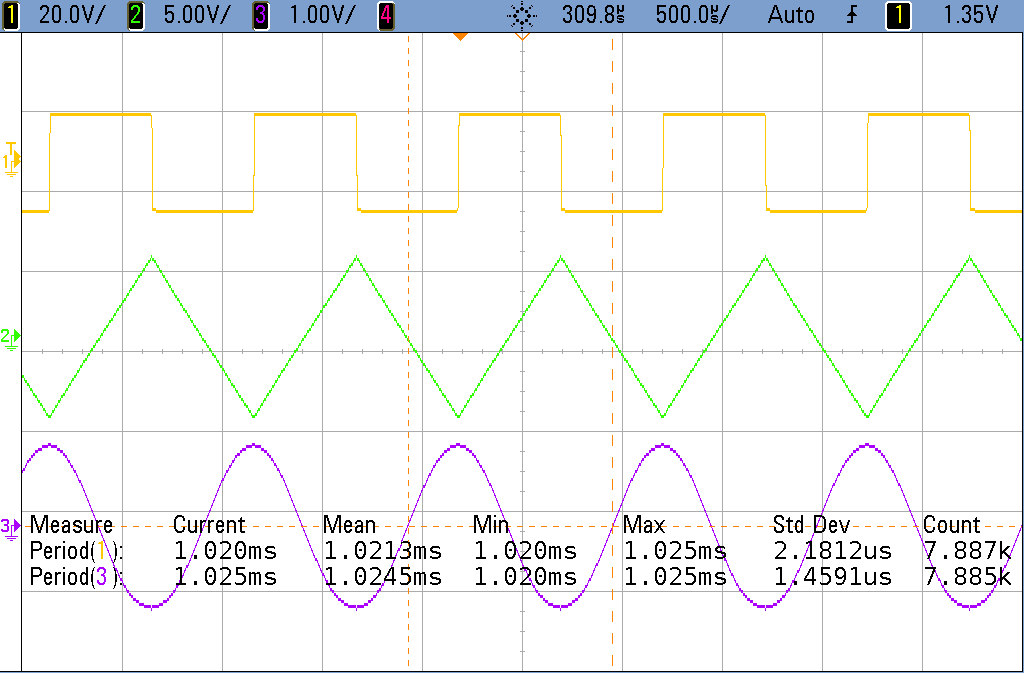
\includegraphics[scale=0.2]{../EJ3/Mediciones/Actuales/Osciloscopio/Jitter/cropped_scope_20.png}
    \end{tabular}    
    \caption{Medida del Jitter medida en el osciloscopio}
    \label{fig:medida_jitter}
\end{figure}

\subsubsection{An\'alisis de resultados}
En primer lugar, existe un error en las frecuencias obtenidas respecto de lo consignado que no se mantiene de forma homog\'enea para todo valor de frecuencia,
lo cual se asume que se debe a la tensi\'on de saturaci\'on del amplificador. Al ser medido se pudo observar que en los extremos existe una ligera diferencia.
Esto se atribuye a las limitaciones de corriente y slew rate del amplificador operacional, con lo cual a mayor frecuencia se puede acrecentar tales variaciones,
modificando los valores l\'imite del comparador que controla la oscilaci\'on. No obstante, este error fue compensado dentro de lo aceptable con la etapa de acondicionamiento lineal.

En segundo lugar, es razonable considerar que las frecuencias bajas tendr\'an mayor error dado que implica una carga del capacitor con corrientes constantes de menor magnitud,
por ende se vuelven m\'as apreciables a los valores de corrientes de bias y offset del amplificador operacional, por ende introduce un error relativo mayor.

En tercer lugar, otro aspecto que introduce error que puede depender de la frecuencia de oscilaci\'on del circuito, es el transistor MOS, ya que su entrada tiene atribuida una capacidad
que requiere un determinado tiempo transitorio para acumular cargas y lograr que se abra el canal de conducci\'on, por lo cual, siempre puede existir un determinado tiempo de retardo que desfasa
la onda cuadrada y la triangular e introduce errores temporales.

Finalmente, los valores de THD de la senoidal de salida se consideran aceptables dentro de lo esperado, no obstante si en vez de utilizar componentes discretos pudieran recrearse condiciones \'optimas
empleando un circuito con mejores relaciones, ya sea de tolerancia o de paridad entre transistores, en te\'oria desde un punto de vista ideal podr\'ia reducirse hasta $0.02\%$.

\subsection{Conclusiones}
El oscilador controlado por tensi\'on es un circuito que permite generar de forma sencilla ondas de frecuencia variable y controladas por una tensi\'on de entrada, cuyo error se puede ver acotado si toman
medidas espec\'ificas para ello como la utilizaci\'on de comparadores de alta velocidad y amplificadores operacionales cuya salida pueda alcanzar la tensi\'on de alimentaci\'on, es decir, rail-to-rail. Luego,
se puede obtener una salida senoidal con una baja distorsi\'on siempre y cuando se garantice que se cumplan mejor las condiciones \'optimas del par diferencial del convertidor. Este circuito garantiza
la generaci\'on de ondas senoidales con frecuencia variable, y puede ser empleado para modulaci\'on en frecuencia y circuitos de PLL.